% uw-wkrpt-se.tex - An example work report that uses uw-wkrpt.cls
% Copyright (C) 2002,2003  Simon Law
% 
% This program is free software; you can redistribute it and/or modify
% it under the terms of the GNU General Public License as published by
% the Free Software Foundation; either version 2 of the License, or
% (at your option) any later version.
% 
% This program is distributed in the hope that it will be useful,
% but WITHOUT ANY WARRANTY; without even the implied warranty of
% MERCHANTABILITY or FITNESS FOR A PARTICULAR PURPOSE.  See the
% GNU General Public License for more details.
% 
% You should have received a copy of the GNU General Public License
% along with this program; if not, write to the Free Software
% Foundation, Inc., 59 Temple Place, Suite 330, Boston, MA  02111-1307  USA
%
%%%%%%%%%%%%%%%%%%%%%%%%%%%%%%%%%%%%%%%%%%%%%%%%%%%%%%%%%%%%%%%%%%%%%
%
% We begin by calling the workreport class which includes all the
% definitions for the macros we will use.
\documentclass[se]{uw-wkrpt}

% We will use some packages to add functionality
\usepackage{graphicx} % Include graphic importing

% Now we will begin writing the document.
\begin{document}

%%%%%%%%%%%%%%%%%%%%%%%%%%%%%%%%%%%%%%%%%%%%%%%%%%%%%%%%%%%%%%%%%%%%%
%% IMPORTANT INFORMATION
%%%%%%%%%%%%%%%%%%%%%%%%%%%%%%%%%%%%%%%%%%%%%%%%%%%%%%%%%%%%%%%%%%%%%


%% First we, should create a title page.  This is done below:
% Fill in the title of your report.
\title{Development of an iOS Application}

% Fill in your employer's name.
\employer{Crouton Labs Incorperated}

% Fill in your employer's city and province.
\employeraddress{Kitchener, ON}

% Fill in your term.
\term{2B}

% If you want to specify the date, fill it in here.  If you comment out
% this line, today's date will be substituted.
%\date{April 26, 2003}

% If you are writing a "Confidential 1" report, uncomment the next line.
%\confidential{Confidential-1}

%%%%%%%%%%%%%%%%%%%%%%%%%%%%%%%%%%%%%%%%%%%%%%%%%%%%%%%%%%%%%%%%%%%%%
%% Information that wont change
%%%%%%%%%%%%%%%%%%%%%%%%%%%%%%%%%%%%%%%%%%%%%%%%%%%%%%%%%%%%%%%%%%%%%

\author{Jake Nielsen}

\uwid{20338042}

\address{40 Karch st.,\\*
         Cambridge, ON\ \ N3C 1Y5}

\school{University of Waterloo}

\faculty{Mechanical and Mechatronics Engineering}

\email{jake.k.nielsen@gmail.com}

\program{Mechatronics Engineering}

\chair{Dr.\ Pearl\ Sullivan}

\chairaddress{Mechanical and Mechatronics Engineering Department,\\*
              University of Waterloo,\\*
	      Waterloo, ON\ \ N2L 3G1}



% Now, we ask LaTeX to generate the title.
\maketitle

%%%%%%%%%%%%%%%%%%%%%%%%%%%%%%%%%%%%%%%%%%%%%%%%%%%%%%%%%%%%%%%%%%%%%
%% FRONT MATTER
%%%%%%%%%%%%%%%%%%%%%%%%%%%%%%%%%%%%%%%%%%%%%%%%%%%%%%%%%%%%%%%%%%%%%
%% \frontmatter will make the \section commands ignore their numbering,
%% it will also use roman page numbers.
\frontmatter

% After this, we must create a letter of submission.
\begin{letter}
I have just completed my fourth work term, following my \theterm{} term.
Please find enclosed my first work term report entitled:
``\thetitle'' at \theemployer.  

I am one of the co-founders of Crouton Labs Inc. We make smartphone
apps for restaurants in the Kitchener/Waterloo area. In particular, this
report discusses the development choices that I made as the iOS developer
on our development team while designing and programming the app that we
made for Pita Factory.

I have had no direct assistance from anyone.  I do wish to thank Christophe
Biocca for his invaluable support in learning and working with the objective-c
language. I can say without a doubt that my knowledge of the language, its features,
and coding practices would not be half of what they are today if not for Christophe's
expertise.

% Note that I do not need to type out the boilerplate confirmation,
% nor do I need to write a signature block.  This is generated for me.
% We are now finished with the letter.
\end{letter}

% Next, we need to make a Table of Contents, List of Figures and 
% List of Tables.  You will most likely need to run LaTeX twice to
% get these correct.  The first pass for LaTeX to figure out the
% labels, and the second pass to put in the right references.
\tableofcontents
\listoffigures

\section{Summary}


The purpose of this report is to explain the highlights of the software development
project that I was involved with at Crouton Labs Inc. The project itself was meant
to solve the problem of long line-ups at restaurants, and efficiency of fast food
procuction lines. The report explains the coding
practices that were used during the development process, the challenges that were faced
during development, and the solutions that were implimented to solve those problems.
This report emphasises the importance of using proper design patterns and coding practices
by demonstrating the amount of time saved and the quality that can be achieved by 
adhering to these practices. The final product is one that solves the problem it was
intended to solve, is stable, looks good,
is optimized enough that it feels smooth to interact with, and has very readable code.


%%%%%%%%%%%%%%%%%%%%%%%%%%%%%%%%%%%%%%%%%%%%%%%%%%%%%%%%%%%%%%%%%%%%%
%% REPORT BODY
%%%%%%%%%%%%%%%%%%%%%%%%%%%%%%%%%%%%%%%%%%%%%%%%%%%%%%%%%%%%%%%%%%%%%
%% \main will make the \section commands numbered again,
%% it will also use arabic page numbers.
\mainmatter

% You must have an Introduction
\section{Introduction}\label{sec:intro}

The purpose of this report is to convey the challenges that were faced
during the development of the iOS application that Crouton Labs Inc. 
provides to Pita Factory.

In order to undestand the motivation for writing this app in the first
place, it's important to understand what problem this app is intended
to solve. This app is an attempt to reduce the time spent in fast food restaurants
waiting in line and processing transactions. This should allow for the restaurant
to service more customers and thus increase profits. With this in mind,
this main goals of this app are to allow a user to browse the restaurant's
menu, construct an order that they would like to purchase, and to provide
a means of processing the transaction through the app.

The programming language that was used to accomplish this goal is called
objective-c. Objective-c is syntactically similar to c and smalltalk. Its strange
syntactic combination can be confusing at first, as there are often two
syntactically different ways of achieving exactly the same effect. Objective-c
at first glance does not appear to be much different from c++ in terms
of language features, but upon further inspection it can be seen that 
objective-c is perhaps better compared to a dynamic language. While objective-c
does not fit the true definition of a dynamic language, it has many 
language features that are often associated with dynamic languages. 
Object and class methods can be called by progamatic string construction
of the name of the method, which is refered to as a "selector".
Similarly, subclasses can be refered to via programatic strings. With some work,
classes can even request the names of their subclasses, allowing for
some very powerful programming techniques that will be discussed later in
this report.

This report will discuss the general coding practices that were adhered to
during development, the challenges faced during development, and the solutions
that were implimented to deal with the challenges that arose.

The actual interface flow is not within the scope of this report.
The user interface was designed by a 3rd party designer and was merely
implimented and occaisionally exteneded upon by Crouton Labs.

\section{Coding Practices}

\subsection{Motivation}

The coding practices that were maintained 
during the development process are an extremely
important factor that affected the final product of this development
process. Proper coding 
practices are often dismissed or overlooked by many programmers to
the detriment of their productivity and positive outlook. Adhering to 
good practices make the painful parts of software development much less
frequent and much more bearable.

\subsection{Version Control}

Using version control is the single, most important practice any
good programmer should have. While the choice of version control 
software is hotly debated, I am partial to git. Git is a very
powerful source control system and is also very widely used.
Part of good source control use is having a remote repository.
For this project, www.github.com was used as our remote repository.

All version control software has the concept of small, incrimental
changes that, when put together, move the development of the code-base
forward. In git, these are refered to as commits. It's good practice
to make very small, bite-sized commits. In escence, each commit should
fix one bug, impliment one feature, or add one more logical piece to
the codebase. In this way, if certain features aren't working, or simply
aren't finished, they can be excluded from release builds without any
painful merge conflicts.

If a feature is not trivial to impliment, the feature should be
made on a separate "branch" soas to maintain the small size of commits
while still making sure that it is known that the group of commits are 
associated (and likely dependant on) one another. In this way, if a feature
needs to be included or discluded, this can be done simply by including, or 
discluding the entire branch.

\subsection{Efficientcy vs Simplicity}

This is another widely overlooked and undervalued concept that 
helps immensely during the development process. Many programmers
sacrifice simplicity in favor of efficiency much more often than
they should. While it's important under certain circumstances to
have efficient code, it can be hard to know where optimization would
do the most good, or even if it is necessary. Optimization should
only happen if it becomes a problem. Overly optimized code is indistinguishable
from properly optimized code at runtime, but at development time, 
overly optimized code is much less readable, and will cause pain
for any contributors, or even for the person who did the optimization
in the first place. Hence, optimize only when necessary.

\subsection{Refactoring}

It seems obvious, but refactoring is esscencial to maintaining a usable and agile
codebase. To emphasize the importance that needs to be put into refactoring, the 
codebase for this project has been rewritten little-by-little about 3.3 times.
That is, for every line of code in the codebase, there were 3.3 lines added and deleted.
The general mantra that describes good refactoring is, "refactor early, refactor often".

\subsection{Design Patterns}

Design patterns are widely used methods of solving particular problems that can
come up very frequently in programming problems. It's good to have a large arsenal
of design patterns to call on when developing software. By using patterns that
are widely known, your code will be more readable to someone who has never seen
your code before, but has experience with design patterns. Knowlege of design
patterns can drastically increase the speed at which you arrive at solutions.
This is an area that was not adhered to as rigidly as the other proper coding practices,
but it is something that would have added a lot of value. The aggressive refactoring
resulted in a codebase that makes proper use of design patterns, but it would
have been better to have arrived at them initially.

\section{Challenges and Solutions}

\subsection{Section Structure}

In this section, the challenges that were faced will be introduced and
explained. The solutions that were implimented to solve these problems will
also be discussed. It's worth noting that when the software was being developed, 
the approach that was taken involved itemizing all of the challenges that were 
expected to come up so that all of them could be taken into consideration before 
writing a single line of code. In general, it's good to catch the challenges and
make sure that strategies for dealing with them can be incorporated nicely into
the code base. The earlier a challenge is spotted, the faster and more effectively
it can be solved.

\subsection{Code Testing}

In order to be certain that a software solution is relatively bug-free and stable,
it's often good practice to write unit tests and system tests to make sure that
the software operates as expected. In the case of an iOS application, this becomes
a very difficult thing to do. Most of the bugs that occur in iOS applications are
visual or system-behavioural. Since there is no straightforward way to write system
tests for user interfaces, none were written in this development process. Extensive 
manual testing was done prior to releases to make sure that no breaking bugs were
introduced to the live codebase. The lack of unit tests or automated system tests
meant that all of the other coding practices discussed in the previous section became
extremely important. The manual testing also needed to be extremely thorough to make
absolutely sure that no bugs were pushed to the general public. While somewhat frowned
upon, this method proved to be successful, however without almost obsessive adherence
to proper coding practices it likely would not have worked very well. As it stands, only
one release had a bug that was considered to be breaking, and was a relatively subtle
behavioural bug. In terms of stability, to date, there has never been a crash in a
production build.

\subsection{Object Serialization}

In order to serialize an object to save it to non-volitile memory,
serialization and deserialization methods need to be implimented for each class that
needs to be saved. There are 18 different classes within the codebase that need to
be serializable. This quickly became tedious. In order to solve this problem, a class
was created that utilizes some of the more powerful language features of objective-c.
In particular, objective-c allows classes to programatically reference the values
and the names of their member variables. By utilizing that feature, the class (called AutomagicalCoder)  is able
to cycle through all of its own member variables and store serialize them by encoding them
with their own string name as the key. In this way, any class that subclasses AutomagicalCoder
needn't worry about how to serialize itself, and instead just inherently knows how.

\subsection{User Interface Tools}

There are a lot of similarity between facets of a user interface. Particularly in this
application, there was often need to have a way of displaying a multitude of different
types of objects as cells in a table. Similarly, the behaviour invoked when the user
taps on these object cells with his/her finger is often (although not always) the same.
Both of these problems lent themselves well to the dispatcher design pattern. 

In the dispatcher pattern,
when it is necessary to do a similar action to many different types of data, instead of coding
each action separately, the data is sent to a "dispatcher" that looks through the data that
it knows how to handle, and decides accordingly which special actions to take depending on
the data. If the data is not of a known type, depending on the dispatcher, it is either correct
to take some default action, or simply to throw an error to let the programmer know that 
an unexpected piece of data was passed to the dispatcher. Objective-c lends itself to the 
dispatcher method, because of the language feature that allows a class to look through it's
own subclasses without the subclasses explicitly making themselves known to the parent class.

Without delving any deeper, a solid working knowledge of Apple's API is required to understand
most, if not all of the following paragraphs. An abbreviated explaination of Apple's API can 
be found in Appendix A.

In the case of displaying cells, the parent class (CustomViewCell) looks through it's subclass
and calls the canDisplayData method to query them about the data that it has been presented with.
This is shown in the figure below.

\begin{figure}[h!]
  \caption{Illustration of the Dispatcher Design Pattern}
  \centering
    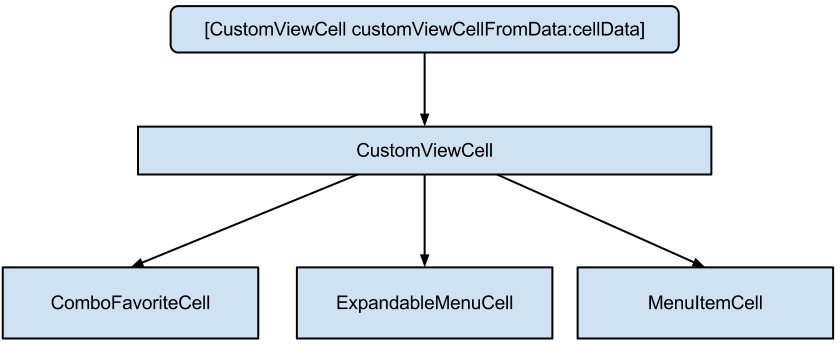
\includegraphics[width=0.5\textwidth]{customViewCellFlowchart}
\end{figure}

In this way, all that is necessary to fully define and display a list view is a list of the data
that should be displayed in the list. By dispatching to CustomViewCell, the particularities of
displaying each individual cell needn't be handled in any way by the tableViewDelegate. 

Another language feature involved in the simplification of the TableView interface provided
by Apple is that of calling methods by constructing their name through string manipulation.
If there's somthing that needs to occur when the user clicks on a cell, the TableViewDelegate
need only impliment a function named <CELLNAME>Handler. The method (if it exists) will be called
by the table view delegate whenever the cell is clicked on. In this way, the delegate can 
distinguish between cell clicks without needing to actually know the type of the cell or the
position of the cell (which is the traditional way that Apple intends for cell distinctions to
be made). 

By making all of these simplifying abstractions, the code length of the files defining
the behaviour of particular pages is vastly. One class in particular (OrderComboViewController)
has 4 lines of code in its header file and 23 lines of code in its implimentation. A screenshot
of this particular page is shown below. 

\begin{figure}[h!]
  \caption{Screenshot of the Order Combo Page}
  \centering
    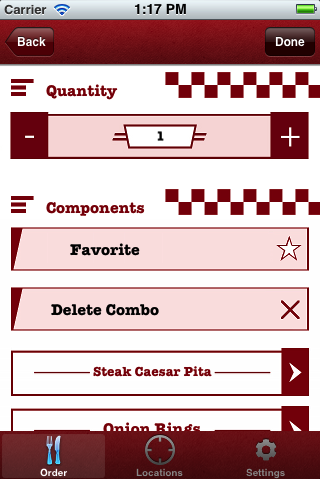
\includegraphics[width=0.5\textwidth]{orderComboPage}
\end{figure}

The UITableViewDataSource for this page is simplified in a similar way. The class responsible
for the page contents (OrderComboRenderer) has 7 lines in its header file, and 37 in its implimentation.


The dispatcher pattern is a very powerful way of simplifying code.

\subsection{Client Version Management}

One of the complicating factors in designing any application is how various versions of the code will
interact with one another. The two possible modes of interaction in this case are communication with
the server, and loading data cached by an older version of the client code. 

\subsubsection{Server Communication}

If an old version of the client code were to try to interact with the server, the server's behavior
may have to be different than if an up to date client app were to attempt communications. The way that
this is solved is again by dispatching. As part of every communication with the server, the iOS application
transmits its version number. Based on the version number, the server dispatches the the response behaviour
to the appropriate version of the server code.

\subsubsection{Client Data Caching}

A more difficult complication is that of loading cached data. If the ipod/iphone user has an old version of the
app, saves some data, updates their app to the current version, and then attempts to load the cached data,
bad things can happen. Depending on the version of the app that was used to cache the data, the procedure
to update the data to be consistant with the current model is different. To solve this problem, a combination
of the dispatcher pattern and the fallthrough pattern was used. The first step in determining what to do
with the data being loaded is to check the version string. Luckillty, this problem was anticipated, and 
the cached data always contains a version string. Because this all needs to be done by AutomagicalCoder,
no actual knowledge of what these variables are is known explicitly at load time. To solve this, Automagical
Coder checks the version string, and if the version string is not the current version string, it checks for
the existance of a recovery routine for each of the variables that it determines that it needs to load.
if a recovery routine is implimented in the child class, AutomagicalCoder dispatches to the recovery 
routine by calling <VARIABLENAME>Recovery. The recovery routine uses the fallthrough pattern.

The fallthrough pattern uses a switch case structure where the case clauses do not contain a break statement.
In this way, the variable information will be updated in a cascade through all of the versions starting
at the version that was found on the disc all the way up to the present model. In this way, the only
thing that needs to be updated from version to version is the logic for moving the data from the version
immediately prior to the current version. Everything else just cascades through.

\section{Conclusion}

In conclusion, by using the habits and patterns discussed in this report, the development project was a 
great success. From a technological view point, this product turned out great. It's stable, it looks good,
it is optimized enough that it feels smooth to interact with, and its code is very readable. 

The app can currently be downloaded from the app store, and is called "Pita Factory". As
not everyone has an iOS device, below are some screenshots of the finished product.

\begin{figure}[h!]
  \caption{Screenshot of the Order/Menu Page}
  \centering
    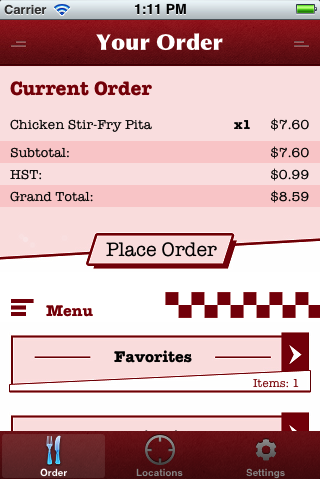
\includegraphics[width=0.5\textwidth]{orderMenuPage}
\end{figure}

\begin{figure}[h!]
  \caption{Screenshot of the Credit Card Page}
  \centering
    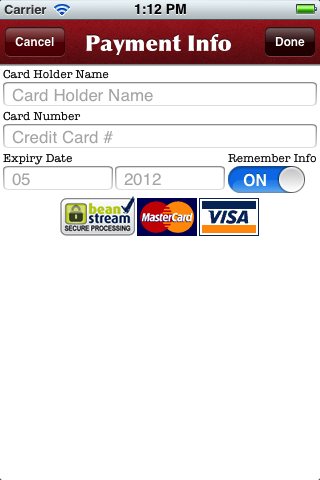
\includegraphics[width=0.5\textwidth]{creditCardPage}
\end{figure}

\begin{figure}[h!]
  \caption{Screenshot of the Location Page}
  \centering
    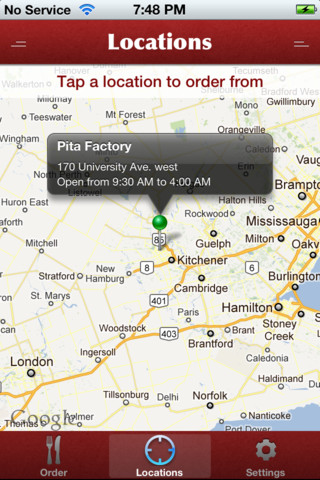
\includegraphics[width=0.5\textwidth]{locationPage}
\end{figure}

\appendix

\section{Apple API Abbreviated}

Appendix A is an abbreviated description of Apples's iOS API. It
will explain the general concepts behind displaying things on
an iOS device as well as the specific elements of the API that
are pertainant to this report.

As a general overview, there are views, models, and controllers.
The views represent the actual images that the user sees. The models
represent the data that is meant to be conveyed to the user. The
controllers encapsulate the ways that the user can interact with
the data. This is known as the model-view-controller design pattern
and is the design pattern that apple intends for programmers to use
when interacting with their API.

\subsection{UIViews}

UIView is the most basic class that is meant to be displayed to
the screen. A UIView has an area of the screen that it can manipulate
via its drawrect method. A UIView can also have an arbitrary number of 
subviews which draw themselves onto the parent UIView. There are 
many built-in subclasses of UIView that can accomodate most 
applications that a person might want to build.

Some notable subclasses of UIView are: UILabel, UIButton, UITableView
UIViewCell, and UIImageView.

\subsubsection{UITableView}

A UITableView is a view that can display any number of scrollable 
UIViewCells. The UITableView must be associated with a UITableViewDelegate
in order to define any interactive behaviour and must be associated
with a UITableViewDataSource in order to have any content. they will be
discussed more in the UIViewControllers and UIDataSources sections.

\subsubsection{UIViewCell}

A UIViewCell is a UIView that can be produced by a UITableViewDataSource.
The vanila UIViewCell can be used by itself as elements to populate a
UITableView and can be configured in several different default configurations
that can accomodate most data that a person might want to display reasonably
well. In cases where the vanila UIViewCell will not suffice, UIViewCell can
be subclassed to accomodate arbitrarily complex and unusual cells.

\subsection{UIViewControllers}

UIViewController is a class that is not intended to be used by itself, 
but rather to be subclassed to accomodate specific behaviour that
a programmer might intend for a view to have. View controllers are
often made to be the delegates of the view that they control so that
a view can request behavior from its view controller without actually
needing to know anything specific about the view controller. 

\subsubsection{UITableViewDelegate}

The most notable type of delegation that this report refers to is
that of the UITableViewDelegate. The UITableViewDelegate is responsible
for telling the UITableView what needs to happen upon the selection of
a cell at a particular position on the table. It's also responsible for 
letting the UITableView know the height that each cell is intended to
occupy.

\subsection{UIDataSources}

In general, the "model" part of the model-view-controller pattern is 
satisfied by a class that impliments a datasource interface defined for
the UIView that it is acting as the model for. This is not always
the case, and in cases where it isn't, the model will simply be a 
subclass of NSObject, which is a base class that everything derrives from
within the the Apple API.

\subsubsection{UITableViewDataSource}

A class that impliments the UITableViewDataSource interface will provide
a UITableView with the cells that the UITableView will populate itself with
as well as letting it know the number of cells that exist in the table,
the titles of the sections that make up the table.


\end{document}
